\documentclass{beamer}
\usepackage [english]{babel}
\usepackage {amssymb}
\usepackage {amsmath}
%\usepackage {beamerthemeBerlin}
\usetheme{Darmstadt}
%\usetheme{Warsaw}
\title{Modelling of oil spills}
\author{
	Alexey Osipov\inst{1, 2}
}
\institute{
	\inst{1}
	Syncretis
	\inst{2}
	Tinkoff
}
\date{October 2023}
\begin{document}
\begin{frame}
\titlepage
\end{frame}	
\begin{section}{Introduction}
\begin{frame}{Statement of the problem}
Examples of oil spills: Deepwater Horizon (2010), Wakashio Oil Spill (2020).	
	
Given high precision satellite images, it is necessary to provide opportunities:
\begin{itemize}
	\item to automatically detect oil spills,
	\item to forecast change of oil spill over time,
	\item to model influence of various parameters on an oil spill,
	\item to forecast past behaviour of the oil spill.
\end{itemize}

\begin{figure}[H]
	\centering
	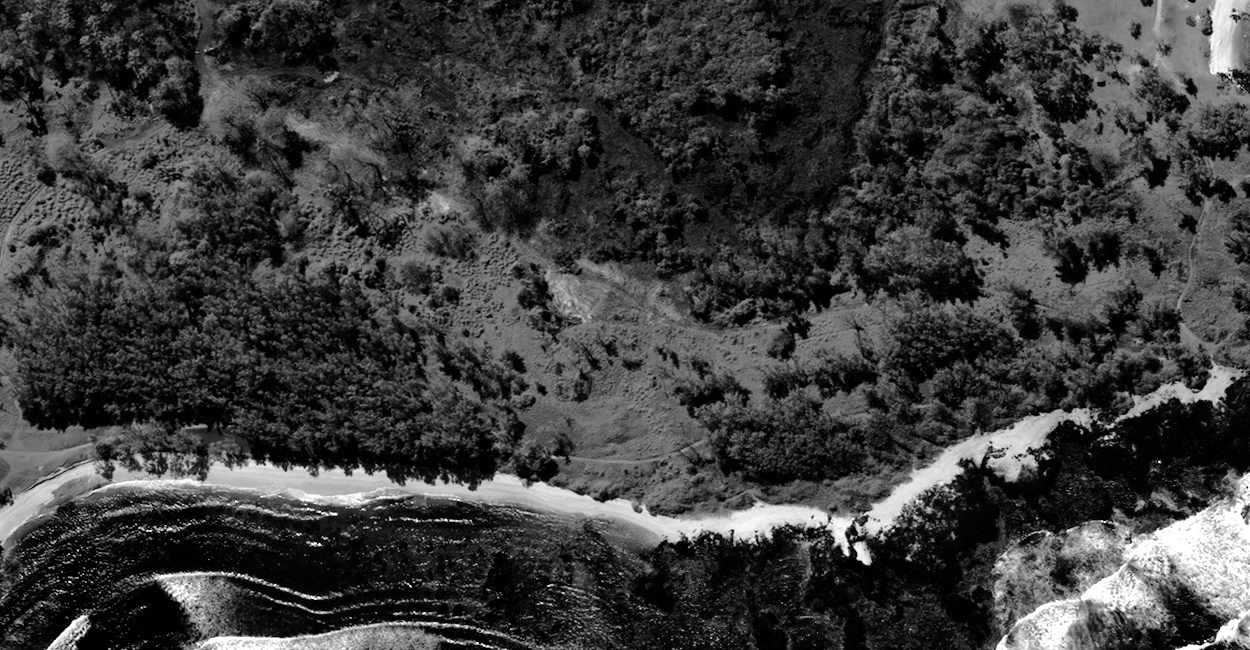
\includegraphics[scale=0.1]{maxar_8thAugust_1_21_45.png}
\end{figure}
\end{frame}
\begin{frame}{OilSync}
\begin{itemize}
	\item \textbf{OilSync} is a software for modelling oil spills that solves the problems stated above,
	\item it is registered in Reestr of Russian Software, register entry №19208 from 23.09.2023.
\end{itemize}

\begin{figure}[H]
	\centering
	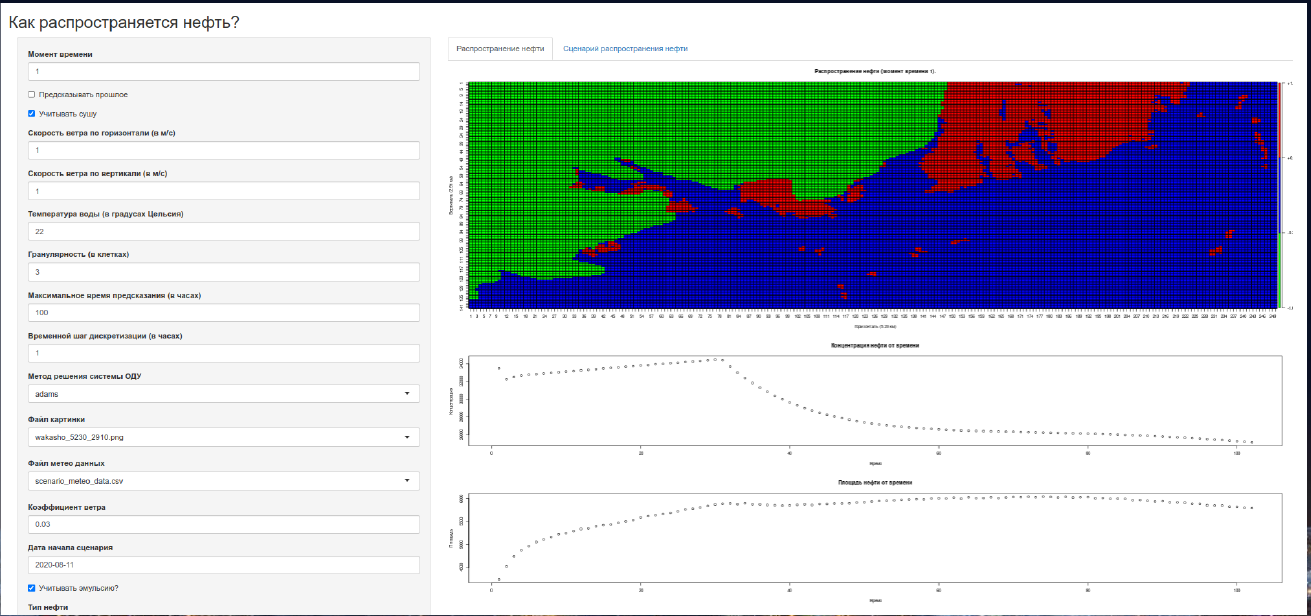
\includegraphics[scale=0.2]{how_oil_spreads.png}
\end{figure}
\end{frame}

\begin{frame}{General scheme of the solution}

\begin{figure}[H]
	\centering
	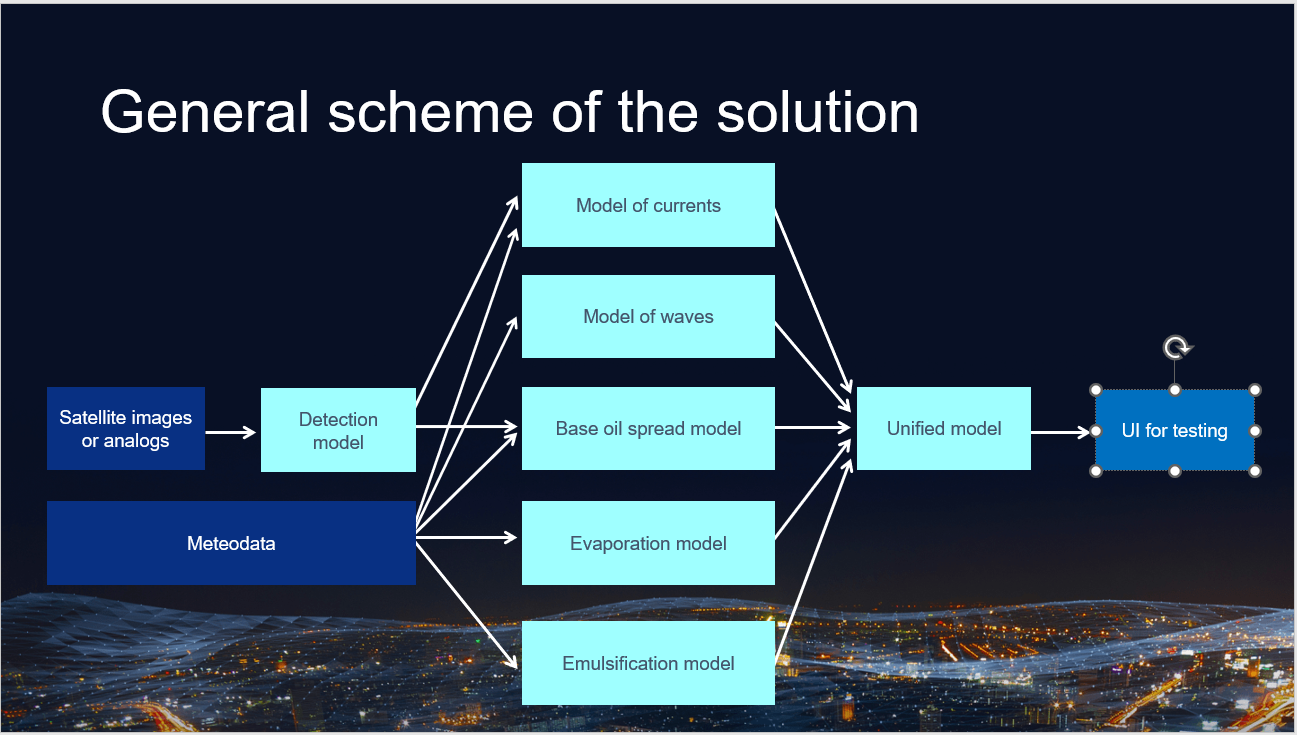
\includegraphics[scale=0.4]{general_scheme_of_the_solution_eng.png}
\end{figure}
	
\end{frame}

\begin{frame}{State of the art}
		
\begin{enumerate}
	\item The detection problem is more or less solved.
	\item The spread problem does not have a good solution due to presence of large number of factors.
	\begin{itemize}
		\item There are open-source solutions (e. g., \textbf{gnome}, \textbf{HyosPy}), there are closed solutions,
		\item \textbf{Euler formulation}, the spill is modelled as a whole,
		\item Lagrange formulation, the spill is modelled as a set of particles.
	\end{itemize}
\end{enumerate}

\begin{figure}[H]
	\centering
	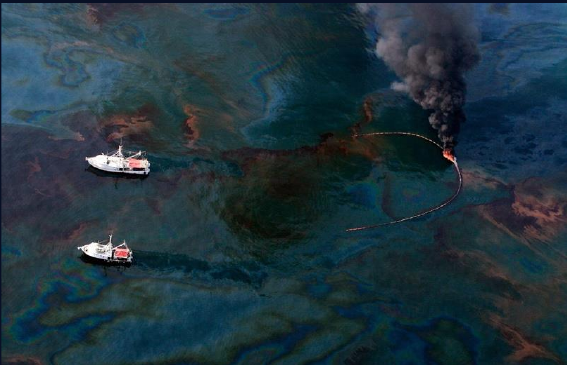
\includegraphics[scale=0.25]{example_oil.png}
\end{figure}
		
\end{frame}

\end{section}

\begin{section}{Detection problem}
	\begin{frame}{Data for detection}
	\begin{itemize}
		\item A dataset for research institutions (https://m4d.iti.gr/oil-spill-detection-dataset/)
		
		\begin{figure}[H]
			\centering
			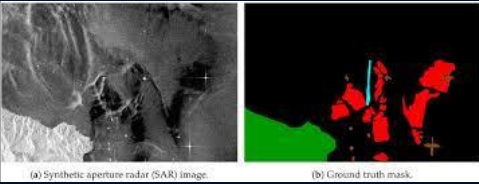
\includegraphics[scale=0.2]{greek_dataset_example.png}
		\end{figure}
		
		\item A dataset of Syncretis: weak labelling (euristics and clustering on data by Maxar)
		
		\begin{figure}
			\centering
			\begin{minipage}{0.5\textwidth}
			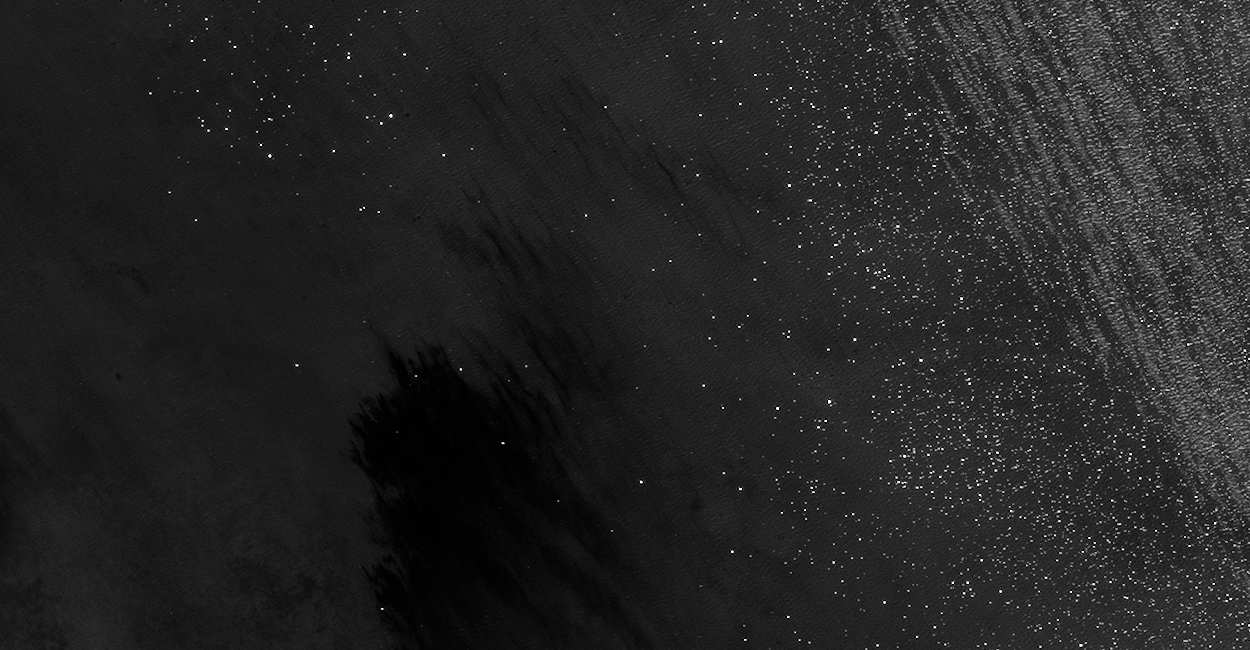
\includegraphics[scale=0.1]{maxar_8thAugust_1_26_28.png}
			\end{minipage}%
		    \begin{minipage}{0.5\textwidth}
		    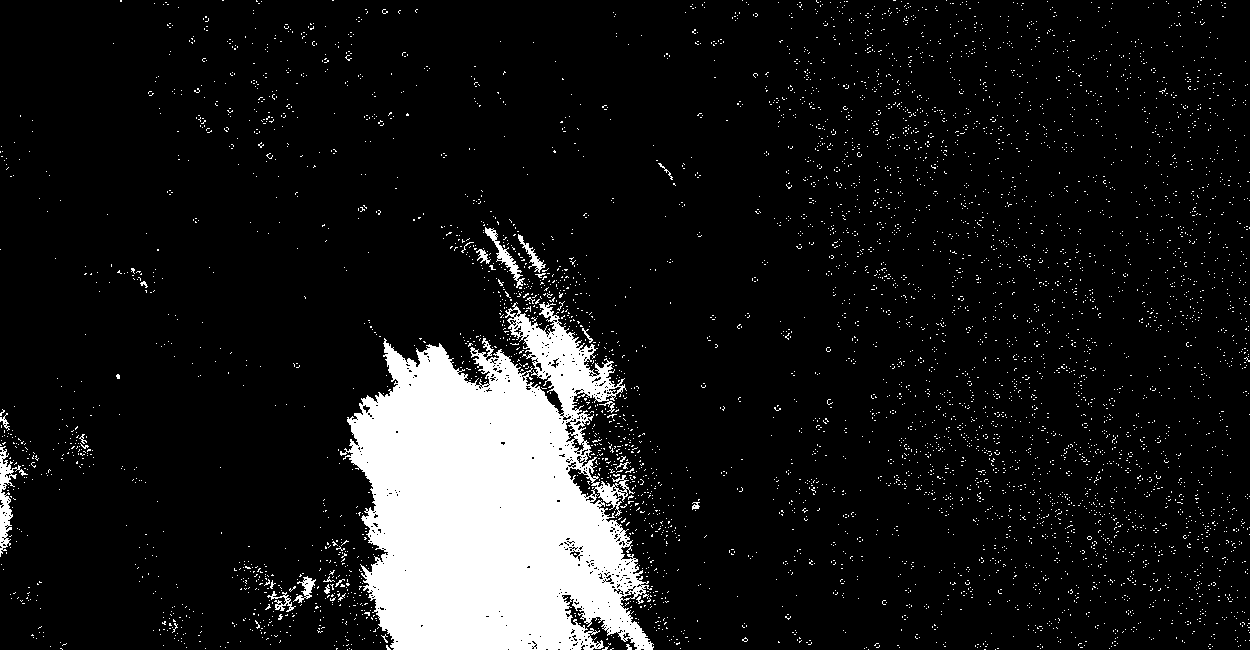
\includegraphics[scale=0.1]{maxar_8thAugust_1_26_28_mask.png}
		    \end{minipage}
	    \end{figure}
	
	\end{itemize}
	\end{frame}

\begin{frame}{DeepLabV3+}
\begin{figure}[H]
\centering
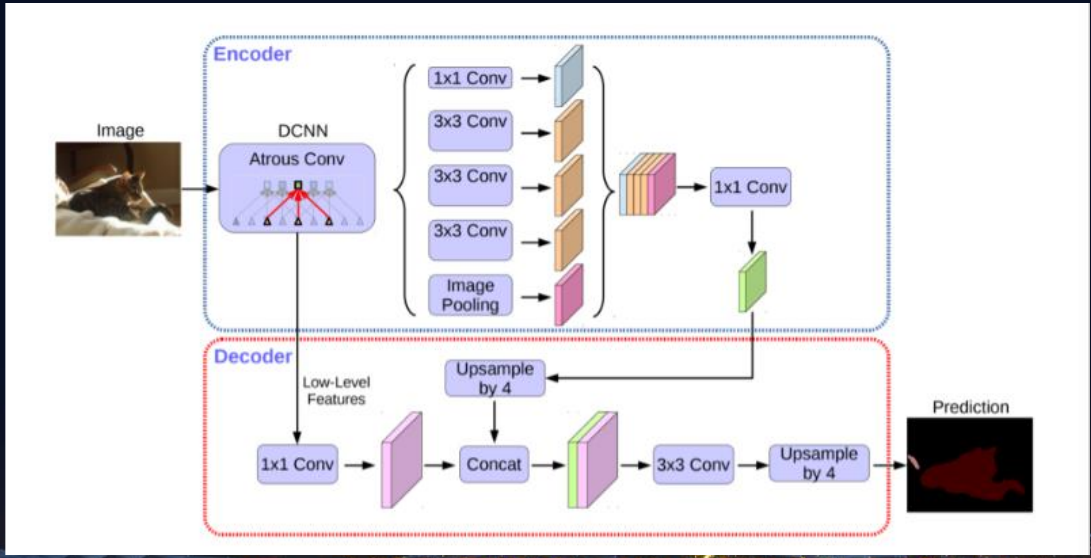
\includegraphics[scale=0.25]{deeplabv3plus.png}
\end{figure}
\end{frame}

\begin{frame}{Detection model}
	\begin{itemize}
		\item Best models from papers by \textbf{Krestenitis et al}:
		\begin{enumerate}
			\item DeepLabV3+ with ResNet101,
			\item DeepLabV3+ with MobileNetV2,
			\item UNet.
		\end{enumerate}
	    \item Detection model by Syncretis:
	    DeepLabV3+ with ResNet50,
	    \item In all cases mean IoU is around 0.65.
	\end{itemize}

\begin{figure}[H]
	\centering
	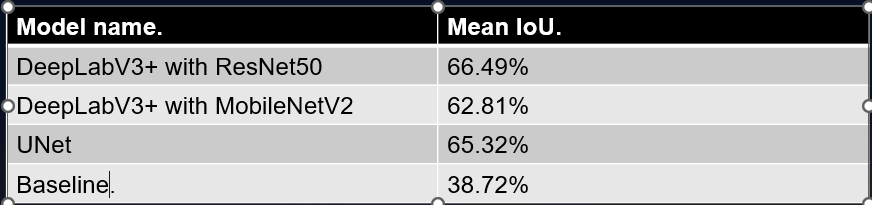
\includegraphics[scale=0.6]{table_1_eng.png}
\end{figure}

\end{frame}

\begin{frame}{Examples of results}
\begin{figure}[H]
	\centering
	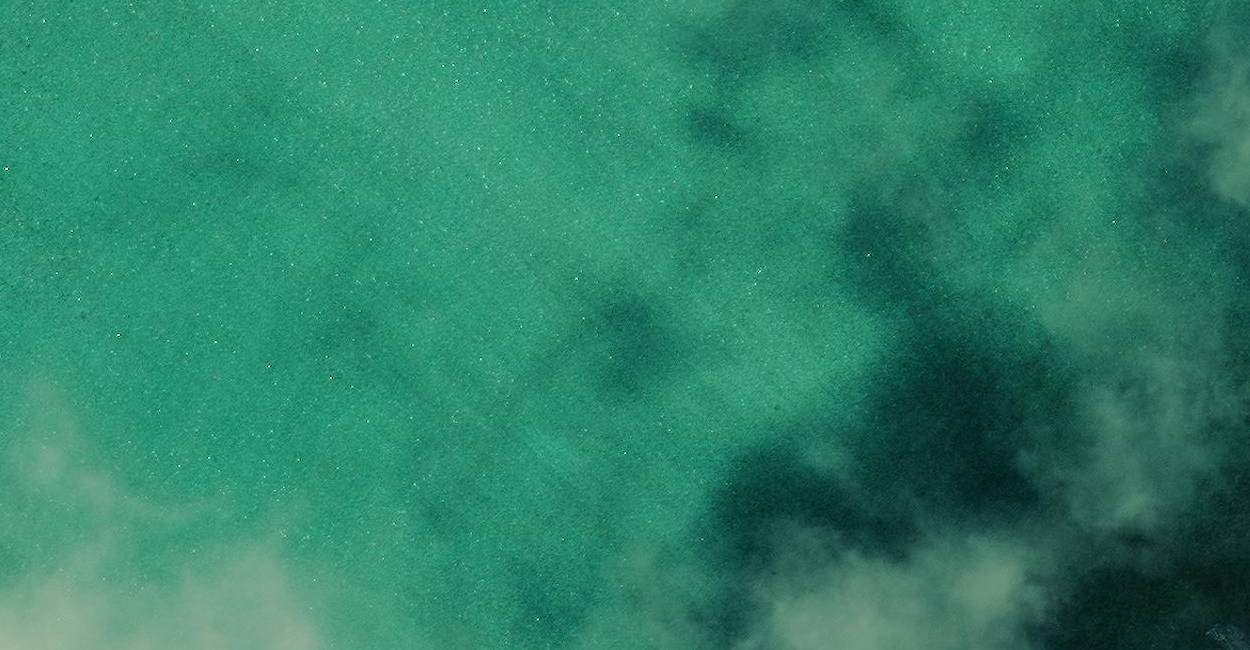
\includegraphics[scale=0.1]{maxar_maxar_16th_October_27_217_image.png}
\end{figure}

\begin{figure}
	\centering
	\begin{minipage}{0.5\textwidth}
		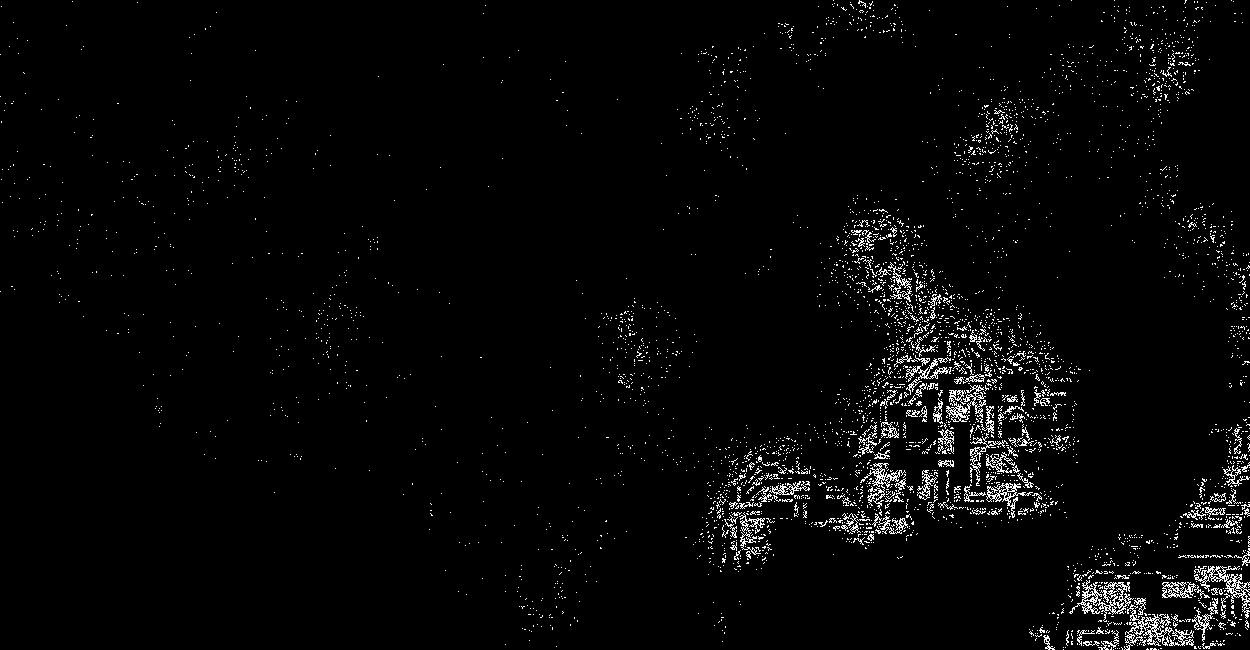
\includegraphics[scale=0.1]{maxar_maxar_16th_October_27_217_mask.png}
	\end{minipage}%
	\begin{minipage}{0.5\textwidth}
		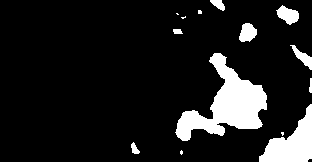
\includegraphics[scale=0.4]{maxar_maxar_16th_October_27_217_results.png}
	\end{minipage}
\end{figure}

\end{frame}

\end{section}
\begin{section}{Oil spread model}
\begin{frame}{Input data}
\begin{itemize}
\item Wind velocity (vector).
\item Water temperature (for coefficient of diffusion).
\item Data on the spill and on the land.
\item Data on time.
\end{itemize}
Dynamical system.

\begin{figure}
	\centering
	\begin{minipage}{0.5\textwidth}
		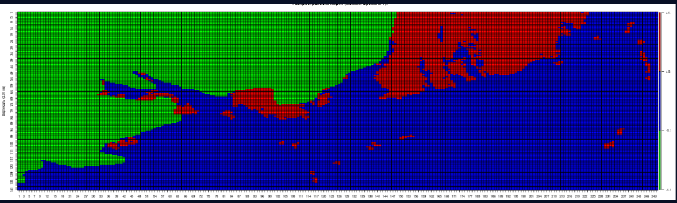
\includegraphics[scale=0.2]{photo_before.png}
	\end{minipage}%
	\begin{minipage}{0.5\textwidth}
		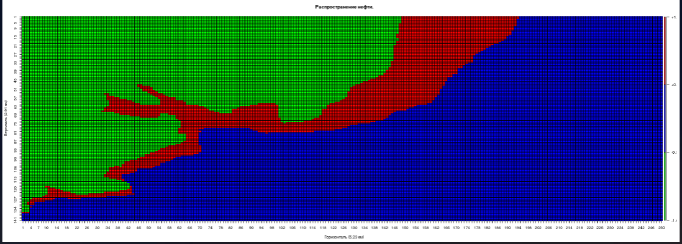
\includegraphics[scale=0.2]{photo_after.png}
	\end{minipage}
\end{figure}

\end{frame}		
\begin{frame}{Base model}
\begin{itemize}
	\item Advection-diffusion reaction on concentration:
	
	$$\frac{\partial C}{\partial t} + u\cdot\nabla C = \nabla (k\nabla C),$$
	$$k = 0.002\left(\frac{T}{22}\right)^{1.53}.$$
	
	\item Boundary conditions correspond to the detected spill.
	
	\item Discretization and reduction to a system of ODEs.
	
	\item Solution of ODE system by method of Adams.
	
	\item The model is taken from \textbf{Duran et al}.
	
\end{itemize}
\end{frame}

\begin{frame}{Features of the base model}
\begin{itemize}
	\item Wind velocity may depend on time and on coordinates.
	\item The land is taken into account via a separate script.
	\item The inverse problem for the model is not solvable, but it is solvable for the approximation. 
\end{itemize}

\begin{figure}[H]
	\centering
	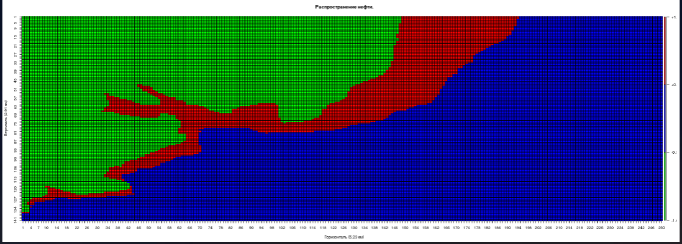
\includegraphics[scale=0.2]{photo_after.png}
\end{figure}
\end{frame}

\begin{frame}{Data for the model of currents}
\begin{itemize}
	\item Data on currents by \textbf{Woods Hole Oceanographic Institution}.
	\item Short time series.
	\item Dependency on geographical coordinates.
	\item Annual data.
\end{itemize}

\begin{figure}[H]
	\centering
	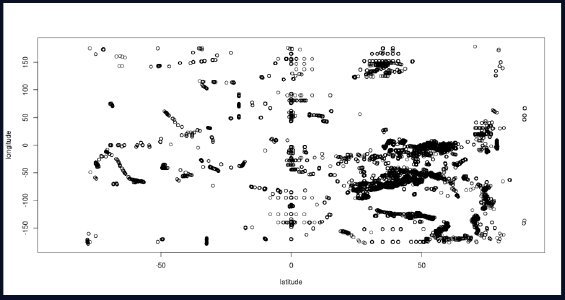
\includegraphics[scale=0.3]{scatter_plots_on_currents.png}
\end{figure}
\end{frame}

\begin{frame}{Forecast of the model of currents}
\begin{itemize}
	\item Solution components: euristics, HDBSCAN, SMA, EMA, Catboost, VAR.
	\item The model: blending of models basing on HDBSCAN, EMA, VAR.
	\item MAPE is around 0.45.
	\item Approximation of a point by cluster average during the forecast.
\end{itemize}

\begin{figure}[H]
	\centering
	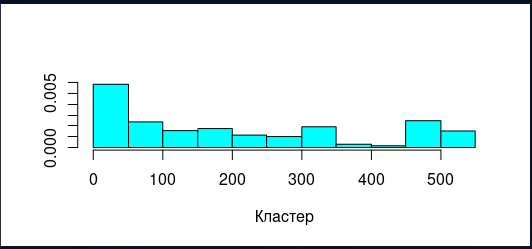
\includegraphics[scale=0.3]{histogram_on_currents.png}
\end{figure}

\end{frame}

\begin{frame}{Choice of model of currents}

\begin{figure}[H]
	\centering
	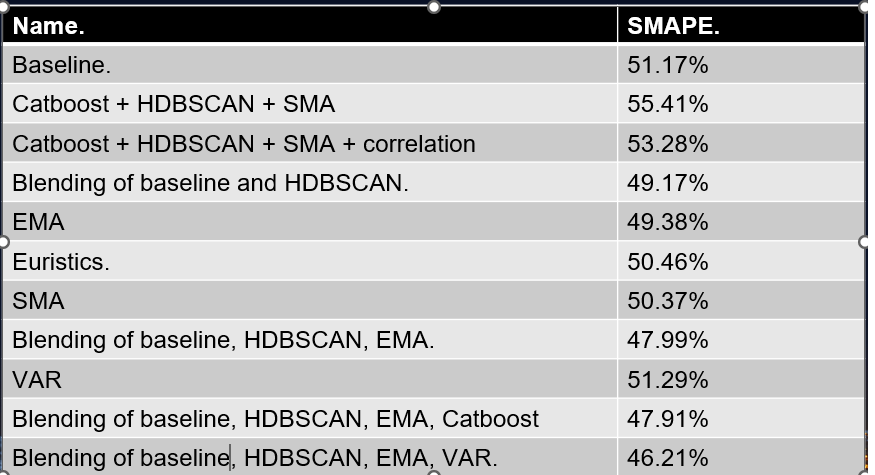
\includegraphics[scale=0.6]{table_2_eng.png}
\end{figure}

\end{frame}

\begin{frame}{Model of waves}
\begin{itemize}
	\item The model by Sverdrup, Munk, Bretschneider.
	\item Empirical model basing on wind velocity and fetch length:
	$$H = 0.283\alpha \frac{W^2}{g}\tanh\left(\frac{0.0125}{\alpha}\left(\frac{gF}{W^2}\right)^{0.42}\right),$$
	$$T = 7.54\beta\frac{W}{g}\tanh\left(\frac{0.077}{\beta}\left(\frac{gF}{W^2}\right)^{0.25}\right),$$
	$$\alpha = \tanh\left(0.53 \left(\frac{gH}{W^2}\right)^{0.75}\right),\quad \beta = \tanh\left(0.833\left(\frac{gH}{W^2}\right)^{0.375}\right),$$
	where $H$ is wave length, $T$ is wave period, $W$ is wind speed, $F$ is fetch length.
\end{itemize}
\end{frame}

\begin{frame}{Evaporation model}
The model is taken from \textit{Fingas}:
$$E = KCU^{7/9}d^{-1/9}\textrm{Sc}^{-r},$$
\begin{itemize}
	\item $K$ is mass transfer rate,
	\item $C$ is concentration of oil,
	\item $U$ is wind speed,
	\item $d$ is area of the poll,
	\item Sc is Schmidt number,
	\item $r$ is an empirical constant. 
\end{itemize}
\end{frame}

\begin{frame}{Emulsification model}
Emulsification is a process of mixing of oil and water.

The model is taken from \textit{Aghajanloo et al}:
$$\frac{\partial D}{\partial t} = K \left(1 + U\right)^2\left(\frac{1 - F}{OC}\right),$$
\begin{itemize}
	\item $K$ is emulsification coefficient, 
	\item $U$ is wind speed,
	\item $OC$ is a constant that characterizes type of oil.
\end{itemize}
\end{frame}

\begin{frame}{Vertical transport model}
\begin{itemize}
	\item The oil goes down, and then it goes up.
	\item Three-dimensional generalization of the base model.
	\item The model is taken from \textit{Aghajanloo et al}.
	\item There is a problem with initial conditions.
\end{itemize}

$$\frac{\partial C}{\partial t} + \frac{\partial u C}{\partial x} + \frac{\partial v C}{\partial y} - \frac{\partial w C}{\partial z} = \frac{\partial}{\partial x}D_x\frac{\partial C}{\partial x} + \frac{\partial}{\partial y}D_y\frac{\partial C}{\partial y} + \frac{\partial}{\partial z}D_z\frac{\partial C}{\partial z},$$

where $C$ is concentration, $u$, $v$ are velocities, $w$ is buoyancy speed, $D_x$, $D_y$, $D_z$ are coefficients of diffusion.
\end{frame}

\end{section}

\begin{section}{Conclusion}

\begin{frame}{Features}
	\begin{itemize}
		\item There are two regimes of work: an individual regime and a scenario regime with possibility of validation on historical events.
		\item There are models of oil detection and oil spread.
		\item The model is quite complicated and quite flexible, it can include extra factors.
		\item The oil spread model is based on Euler formulation unlike Lagrange formulation in most other solutions.
	\end{itemize}
\end{frame}

\end{section}

\begin{frame}{Thank you very much for your attention!}

\begin{block}{My contacts}
\begin{itemize}
	\item my e-mail: osipovav28@googlemail.com
	\item my personal webpage: https://sites.google.com/site/osipovav39/
	\item code repositories: https://github.com/AlexO28
\end{itemize}
\end{block}
\begin{block}{contacts of Syncretis}
\begin{itemize}
	\item e-mail of Syncretis: info@syncretis.ru,
	\item website of Syncretis: https://syncretis.com/ru
\end{itemize}
\end{block}

\end{frame}

\end{document}
